\documentclass[a4paper]{article}

\usepackage[portuguese]{babel}
\usepackage[utf8]{inputenc}
\usepackage[T1]{fontenc}
\usepackage{graphicx}
\usepackage{caption}
\usepackage{anysize}
\usepackage{amsmath}

\usepackage{hyperref}
\hypersetup{
	pdftitle = {CAD - TP2}
	,pdfauthor = {João Ferreira \& José Ribeiro Departamento de Engenharia Informática Universidade De Coimbra \texttt{jpbat@student.dei.uc.pt |  jbaia@student.dei.uc.pt}}
	,pdfborder = {0 0 0}
}

\title{Computação de Alto Desempenho - Trabalho Prático 2}
\author{João Ferreira \& José Ribeiro\\
		Departamento de Engenharia Informática\\
		Universidade de Coimbra\\
		\texttt{jpbat@student.dei.uc.pt | jbaia@student.dei.uc.pt}\\
		\texttt{2009113274 | 2008112181}}
\date{Junho 2013}

\marginsize{3.5cm}{3.5cm}{3cm}{3cm}

\begin{document}
\maketitle

\clearpage

\tableofcontents
\clearpage

\setlength{\parindent}{1cm}
\setlength{\parskip}{0.3cm}

\section{Introdução}
\indent \indent Tal como foi referido no relatório anterior, é cada vez mais díficil aumentar a frequência dos processadores, pelo que se verificou um aumento do número de processadores por computador. No entanto como seria fácil de prever também este aumento tem uma barreira, pelo que existiu a necessidade de apostar em computação distribuida.

Assim aparece o conceito de cluster, um aglomerado de computadores que estão ligados a um switch de alta velocidade o que lhes permite fazer computação distribuida através de, por exemplo, passagem de mensagens entre eles.

Assim aparece a biblioteca \textit{Message Passing Interface}, que nos foi apresentada pelo docente nas aulas teóricas e que vai ser por nós utilizada neste projecto.

Tal como no relatório anterior vai ser explicado o algoritmo utilizado, passando-se depois à análise dos resultados dos testes efectuados.
\clearpage


\section{Ambiente de Testes}
\indent \indent Os testes foram executados nos servidores disponibilizados pelo professor, sendo que pelo que nos foi possível constatar estas são as especificações técnicas de cada um deles:
\begin{description}
	\item [Processador] Intel(R) Xeon(R) CPU E5405 @ 2.00GHz, que possui 2 cores e 12MB de L2 Cache.
	\item [Memória RAM] 3.7GB.
	\item [Sistema Operativo] CentOS 6.3.
\end{description}

Ao longo do período de desenvolvimento fomo-nos deparando com alguns problemas, alguns triviais outros nem tanto, que demoraram algum tempo tanto a apercebermo-nos qual a sua causa como a resolvê-los.

O primeiro destes problemas foi não possuirmos espaço na nossa zona pessoal para conseguir guardar o ficheiro de output. Para o solucionar foi necessário que primeiro conseguissemos perceber que o erro não era causado por falha do envio de mensagens e acima de tudo que não era um erro de lógica no algoritmo, pelo que foi necessário fazer debug da nossa solução, algo que não é de todo trivial num programa distribuido. Como resolução tivemos que procurar uma directoria que não tivesse restrições de espaço e na qual nós tivessemos permisões de escrita. Escolheu-se a directoria: \textit{/tmp/cad-output/}.

Outro problema foi causado pelos próprios estudantes, quando por vezes se iniciavam \texttt{runs} sem que se verificasse se estava alguém a utilizar as máquinas. Para além disto nos levar a ter tempos errados de execução, causava falhas de segmentação, pois não teríamos disponível toda a memória de que precisavamos. Para resolver este problema utilizou-se o \texttt{htop}, ferramenta pedida pelo nosso grupo ao docente, para que se pudesse controlar tanto os níveis de utilização dos \textit{CPU} das 9 máquinas, como os utilizadores que estariam a utilizar de modo a que se pudesse racionalizar o tempo exclusivo de processamento.

Um dos principais problemas que tivemos quando se tentou fazer \textit{fine tune} de alguns valores foi as variações nos tempos de execução, algo que não faziamos ideia do porquê de acontecer. Eventualmente apercebemo-nos de que isto acontecia porque quando o programa tentava escrever por cima de um ficheiro que já existia isso o tornava mais lento. Assim achou-se melhor adicionar à opção de \texttt{run} do \texttt{makefile} o comando para apagar a pasta de \texttt{output} de modo a que não houvesse esse tipo de perda de tempo.
\clearpage


\section{Abordagens}
\subsection{Generalidades}
\indent \indent Uma vez que no primeiro projecto criámos aquilo que achámos ser a melhor solução possível para resolver o problema, a nossa solução passa por correr a nossa versão 1.0 do projecto em cada uma das máquinas, sendo que em cada uma dessas máquinas o projecto vai estar a fazer \textit{matching} às transacções que lhe forem atribuidas e depois enviar os \textit{matches} para o master, que tem como função juntar as respostas de todos os \textit{workers} e escrever para ficheiro.

Após isto foi necessário fazer \textit{fine tune} a alguns valores, como por exemplo qual o tamanho ideal do \textit{buffer} de envio em cada uma das máquinas, ou qual a dimensão do \textit{batch} de trabalhos que minimizava o tempo em que os processadores ficavam parados. Este processo nem sempre se verificou ser fácil, uma vez que por vezes em execuções consecutivas com os mesmos valores chegavam a haver variações de 2 segundos nos tempos de execução (25\%) o que obrigava a um grande número de execuções até que se chegasse a qualquer tipo de conclusão sobre a possível modificação de um valor.

Durante todos os testes efectuados verificou-se com o auxílio de ferramentas como o \textit{htop}, se existiriam mais alunos a utilizar os servidores, e o nível de ocupação dos vários processadores das máquinas utilizadas, de modo a que houvesse certezas sobre a validade dos resultados.
\begin{figure}[h]
	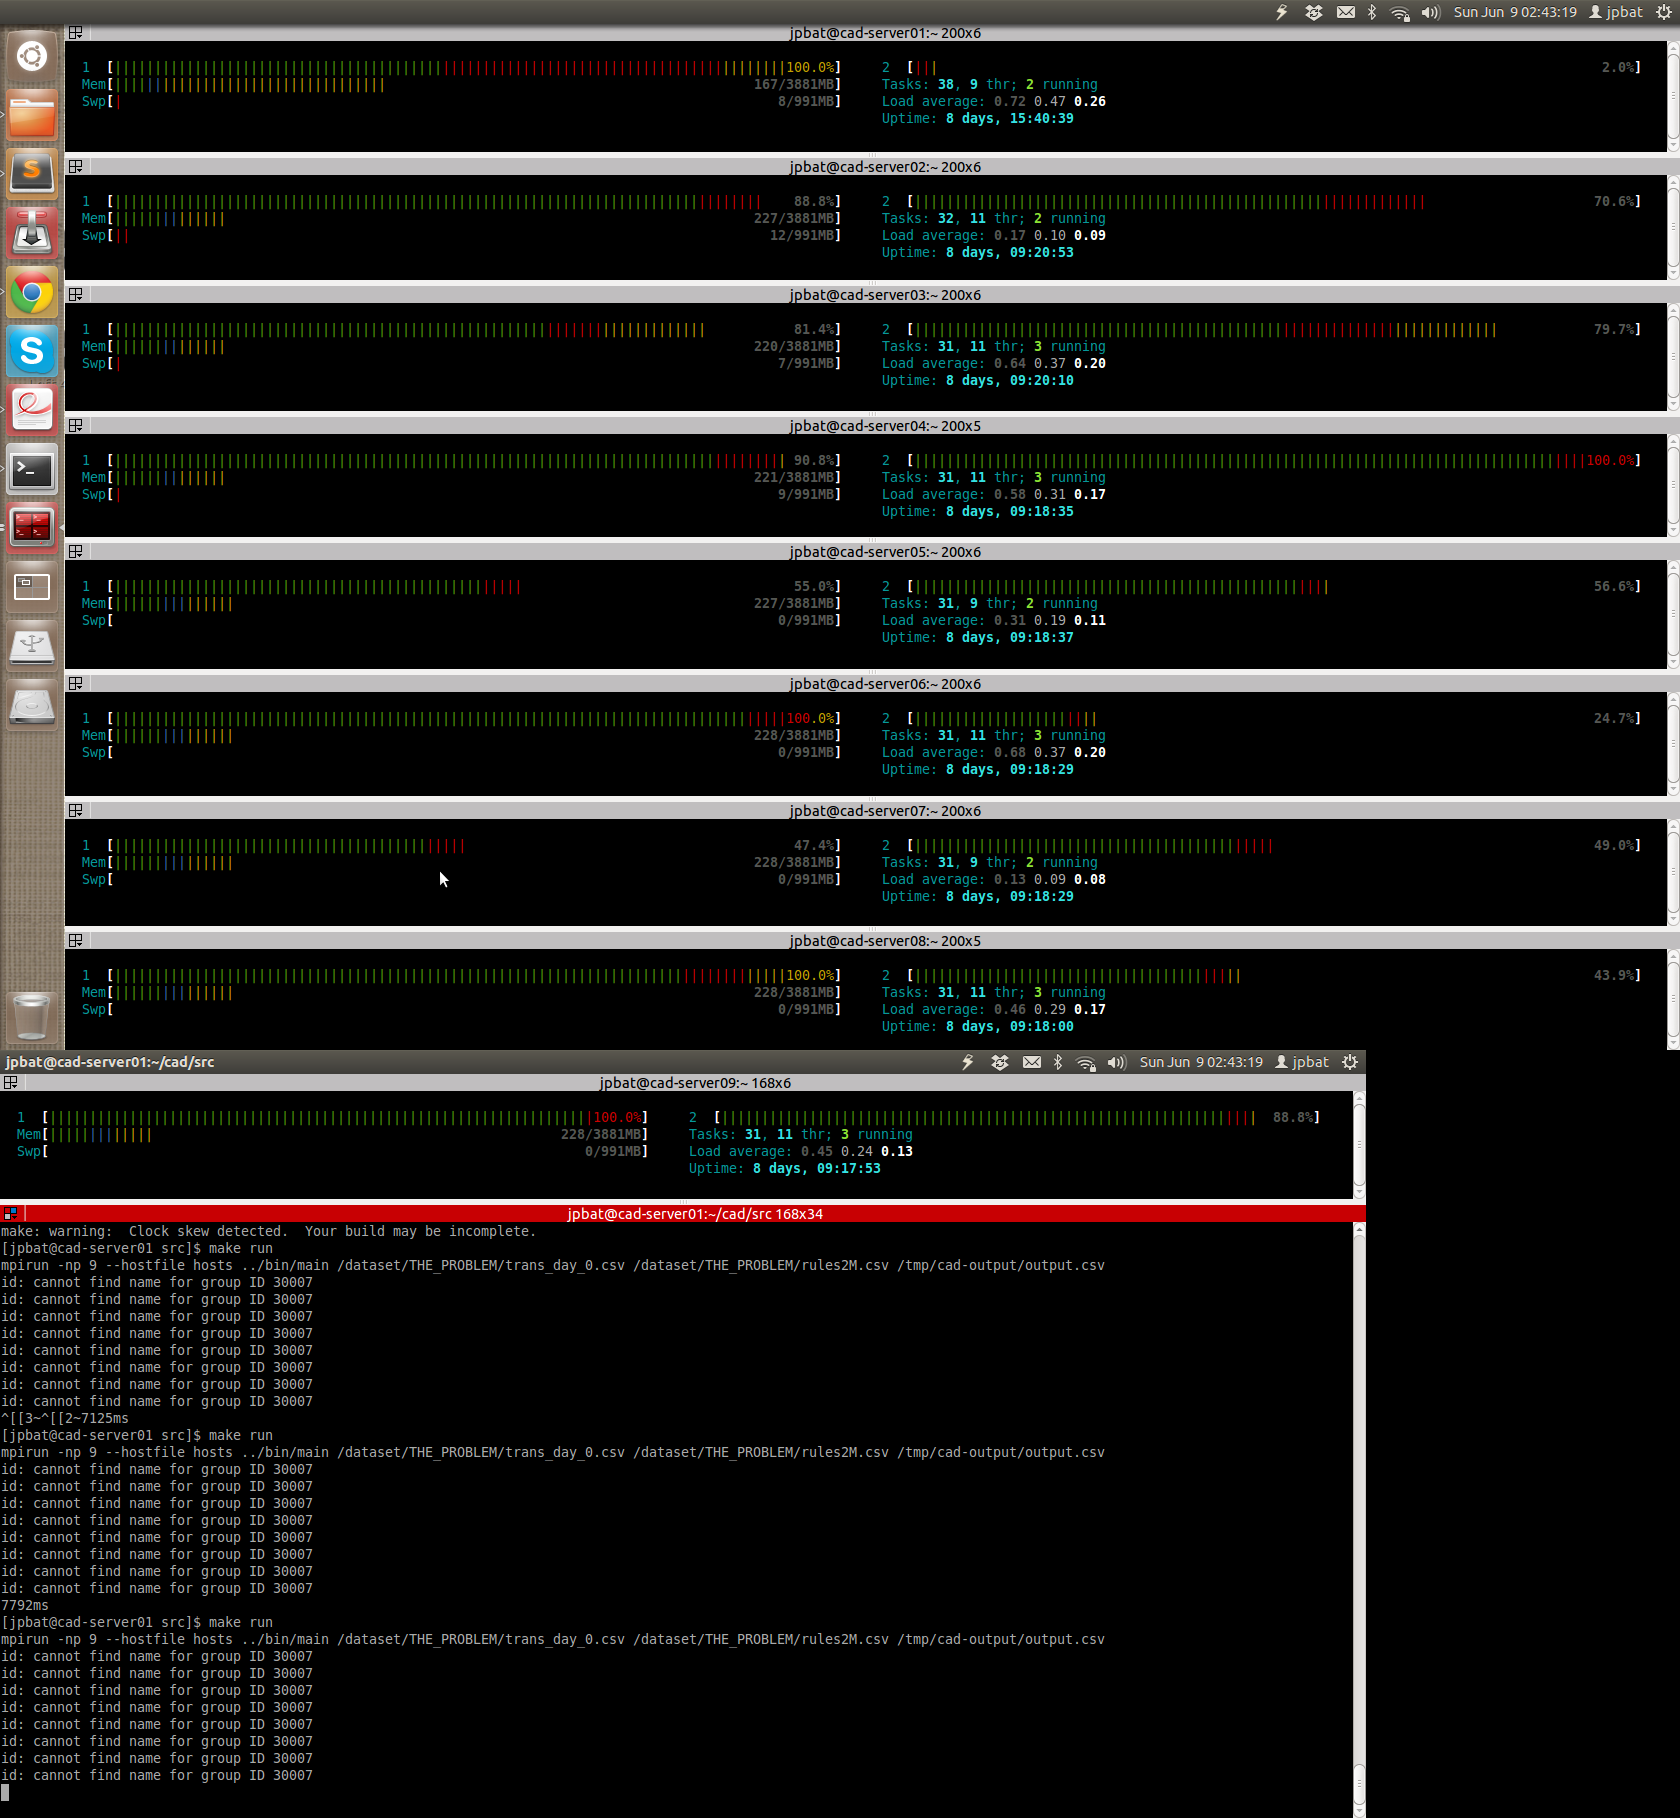
\includegraphics[keepaspectratio=true, width=0.4\textheight]{imgs/ocupacao.png}
	\caption{Monitorização do nível de ocupação dos CPUs.}
\end{figure}

\subsection{Algoritmos}
\subsubsection{V1.0}
\indent \indent Numa primeira versão do algoritmo a começou por se fazer uma distribuição cega do trabalho, ou seja é dado a cada node o mesmo número de transacções sem que haja qualquer tipo de cuidado com um balanceamento de carga.

O node master (MPI\_ID = 0), é single threaded e é responsável por recolher de todos os outros nodes (workers), os matches que estes obtiveram e de os escrever para ficheiro.

Todos os outros nodes têm os índices das transacções que devem tratar, sendo que cada vez que encontram um match vão enchendo um buffer, até que quando este estiver cheio o enviam ao master. 
\subsubsection{V2.0}
\indent \indent Tenho medo do que for para escrever aqui.

Este algoritmo segue o mesmo principio que o anterior, sendo que a grande alteração é baseada no facto de a distribuição de trabalhos não ser cega. Ao invés disso cada node vai pedindo trabalho ao master, de modo a que haja um melhor balanceamento da carga de trabalho.
\clearpage


\section{Resultados}
\indent \indent No primeiro projecto conseguiu-se atingir uma performance de 200000 transacções por segundo numa máquina com seis cores, sendo que nesta a performance do nosso melhor algoritmo não foi além de X. Existem várias razões que podem justificar estes resultados. Neste segundo projecto as nove máquinas a que temos acesso estão a ser virtualizadas, pelo que mesmo cada uma delas tendo o seu próprio sistema de ficheiros, nada garante que fisicamente os ficheiros não estão no mesmo disco rígido, havendo assim um possível \textit{bottleneck} nos acessos a disco. Outra razão que pode explicar estes resultados é o facto de a máquina master ser \textit{single threaded}, pelo que é perdido muito tempo em operações de \texttt{MPI IO}. Por fim o facto de haver alguma, ainda que pouca, latência nas comunicações feitas pela rede pode também ajudar a explicar a performance da nossa solução.

\begin{figure}[h]
	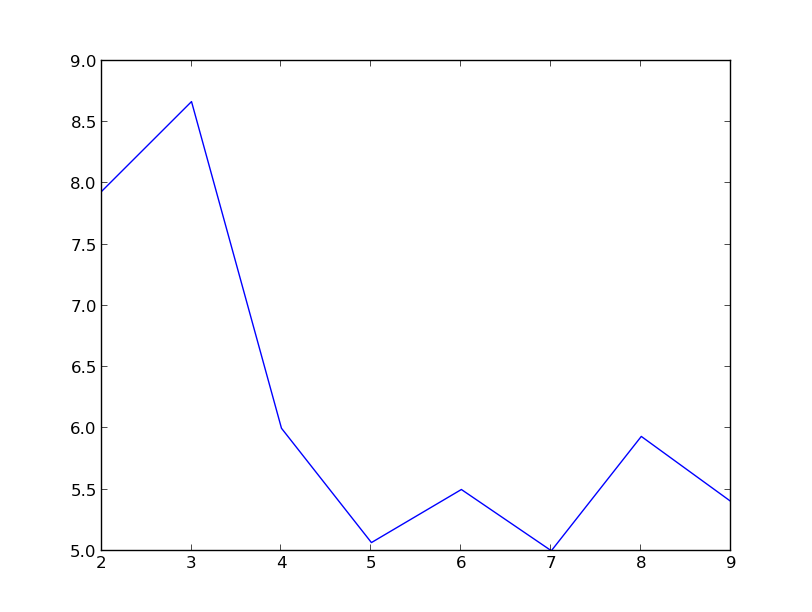
\includegraphics[keepaspectratio=true, width=0.6\textheight]{imgs/scalability.png}
	\caption{Tempo de execução em função do número de nós.}
\end{figure}
\clearpage


\section{Conclusão}
\indent \indent Com o fim do projecto, já depois de termos reflectido sobre todos os dados que foram recolhidos, chega por fim a altura em que se tiram conclusões.

Com este projecto aprendemos que o mundo da virtualização de máquinas tem os seus pontos positivos e os seus pontos negativos. É realmente fácil ``criar'' máquinas mas por vezes é pago a peso de ouro o custo dos acessos ao hardware limitado.

Além disto aprendemos que ter um supercomputador não significa necessáriamente ter um computador com um poder de processamento gigantesco, mas que pode significar também pegar em meia dúzia de computadores francamente mais fracos e ligá-los em rede. Existem claramente vantagens em termos financeiros, sendo que por outro lado é algo mais díficil de programar e sobretudo fazer debug numa arquitectura distribuida.
\clearpage
\end{document}
